%%%%%%%%%%%%%%%%%%%%%%%%%%%%%%%
%This is the article LaTeX template for RSC journals
%Copyright The Royal Society of Chemistry 2010
%%%%%%%%%%%%%%%%%%%%%%%%%%%%%%%

\documentclass[8.5pt,twoside,twocolumn]{article}
\oddsidemargin -1.2cm
\evensidemargin -1.2cm
\textwidth 18cm
\headheight 1.0in
\topmargin -3.5cm
\textheight 22cm
\usepackage[super,sort&compress,comma]{natbib} 
\usepackage{mhchem}
\usepackage{times,mathptmx}
% \usepackage{times}
% feel free not to use mathptmx if it causes difficulties
\usepackage{sectsty}
\usepackage{balance} 

\usepackage{graphicx} %eps figures can be used instead
\usepackage{lastpage}
\usepackage[format=plain,justification=raggedright,singlelinecheck=false,font=small,labelfont=bf,labelsep=space]{caption} 
\usepackage{fancyhdr}
\pagestyle{fancy}

\begin{document}

\thispagestyle{plain}
\fancypagestyle{plain}{
\fancyhead[L]{Communication}
\fancyhead[C]{\hspace{-1cm}
\includegraphics[height=20pt]{headers/CH}}
\fancyhead[R]{Sience Chemistry\vspace{-0.2cm}}
\renewcommand{\headrulewidth}{1pt}}
\renewcommand{\thefootnote}{\fnsymbol{footnote}}
\renewcommand\footnoterule{\vspace*{1pt}% 
\hrule width 3.4in height 0.4pt \vspace*{5pt}} 
\setcounter{secnumdepth}{5}



\makeatletter 
\def\subsubsection{\@startsection{subsubsection}{3}{10pt}{-1.25ex plus -1ex minus -.1ex}{0ex plus 0ex}{\normalsize\bf}} 
\def\paragraph{\@startsection{paragraph}{4}{10pt}{-1.25ex plus -1ex minus -.1ex}{0ex plus 0ex}{\normalsize\textit}} 
\renewcommand\@biblabel[1]{#1}            
\renewcommand\@makefntext[1]% 
{\noindent\makebox[0pt][r]{\@thefnmark\,}#1}
\makeatother 
\renewcommand{\figurename}{\small{Fig.}~}
\sectionfont{\large}
\subsectionfont{\normalsize} 

\fancyfoot{}
\fancyfoot[LO,RE]{\vspace{-7pt}Oregon State University 2017}
\fancyfoot[CO]{\vspace{-7.2pt}\hspace{12.2cm}Sience Chemistry}
\fancyfoot[CE]{\vspace{-7.5pt}\hspace{-14.5cm}\includegraphics{headers/RF}}
\fancyfoot[RO]{\footnotesize{\sffamily{1--\pageref{LastPage} ~\textbar  \hspace{2pt}\thepage}}}
\fancyfoot[LE]{\footnotesize{\sffamily{\thepage~\textbar\hspace{3.45cm} 1--\pageref{LastPage}}}}
\fancyhead{}
\renewcommand{\headrulewidth}{1pt} 
\renewcommand{\footrulewidth}{1pt}
\setlength{\arrayrulewidth}{1pt}
\setlength{\columnsep}{6.5mm}
\setlength\bibsep{1pt}

\twocolumn[
  \begin{@twocolumnfalse}
\noindent\LARGE{\textbf{Identification of an unknown disubstituted benzene derivative}}
\vspace{0.6cm}

\noindent\large{\textbf{Elliott Capek,\textit{$^{a}$} Steven Nguyen,\textit{$^{b\ddag}$} Kristin Ziebart,\textit{$^{b\ddag}$} Kevin Gable\textit{$^{b}$}}}\vspace{0.2cm}
%Please note that \ast indicates the corresponding author(s) but no footnote text is required. 


\noindent\textit{\small{\textbf{Received 22\textit{$^{nd}$} March 2017, Accepted 27\textit{$^{th}$} March 2017}}}\newline

\vspace{0cm}
%Please do not change this text.

\noindent \normalsize{Small organic molecules give off distinct signals in mass spectrometry (MS) and NMR. MS of an unknown disubstituted benzene (codename \textit{Sample 8}) produces a spectra indicating a mass of $136$ atomic mass units (amu). $^{13}$C NMR suggests a total of 8 carbons present in the molecule, six being aromatic, one carboxylic and the other methyl. $^{1}$H-NMR and analysis of molecular mass confirm \textit{Sample 8} as a likely methyl benzoic acid. $^{1}$H-NMR splitting patterns, namely a lack of a singlet peak and presence of four unique aromatic hydrogens, suggest the \textit{meta} substitution pattern. $^{13}$C-$^{1}$H HMBC and HSQC experiments validate this designation. Thus \textit{Sample 8} is given the designation \textit{3-methylbenzoic acid}.}
\vspace{0.5cm}
 \end{@twocolumnfalse}
  ]


\section{Introduction}
%Footnotes

%Please use \dag to cite the ESI in the main text of the article.
%If you article does not have ESI please remove the the \dag symbol from the title and the above footnotetext.

\footnotetext{\textit{$^{a}$~Department of Physics, Oregon State University, Corvallis, Oregon, USA. E-mail: capeke@oregonstate.edu}}
\footnotetext{\textit{$^{b}$~Department of Chemistry, Oregon State University, Corvallis, Oregon, USA}}
\footnotetext{\textit{\ddag~ Authors contributed equally to this work.}}

%additional addresses can be cited as above using the lower-case letters, c, d, e... If all authors are from the same address, no letter is required

Mass spectrometry (MS) and NMR are invaluable techniques for structure elucidation of unknown organic molecules. When a molecule is sufficiently simple, knowledge of its molecular weight, carbon number, and rough identity of carbons and hydrogens can be enough to uniquely determine identity. For more complex molecules, or those with many isomers, further information from 2D experiments like $^{13}$C-$^{1}$H HSQC or $^{13}$C-$^{1}$H HMBC may be necessary.\\

This article follows the designation of a disubstituted benzene unknown using the above techniques. MS is used to determine weight, $^{13}$C NMR is used to come up with a candidate structure, $^{1}$H NMR is used to verify this candidate and guess its substitution, and $^{13}$C-$^{1}$H HSQC is used to verify the substitution.\\

\section{MS}
Molecular mass is first determined by examining the MS spectra shown in Figure \ref{fig:MS}. The largest peak in the highest M/Z ratio peak group is at 136 M/Z, indicating the molecular weight of the unknown is 135 g/mol.\\

The intensity ratio of the major 136 peak and the 137 peak is 0.89, which matches with the theoretical ratio of $0.011*8 = 0.88$ for an 8-carbon molecule.\\

\begin{figure}[h]
\centering
  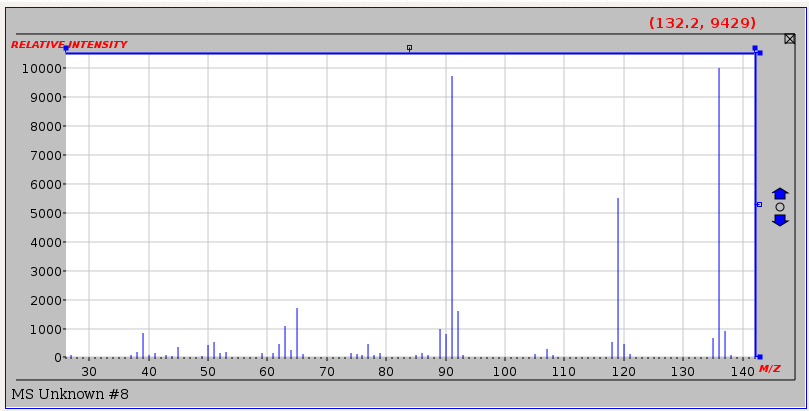
\includegraphics[height=5cm]{figures/MS.png}
  \caption{Mass spectrometry spectra of \textit{Sample 8}.}
  \label{fig:MS}
\end{figure}

\section{$^{13}$C NMR}
The $^{13}$C NMR spectra shown in Figure \ref{fig:CNMR} has 9 peaks. As shown in Table \ref{table:MS}, one peak is due to a DMSO solvent, six to aromatic carbons, one to a methyl carbon and one to a carboxylic carbon. These results agree with the 8-carbon estimate from peak ratios in MS.\\

\begin{figure}[h]
\centering
  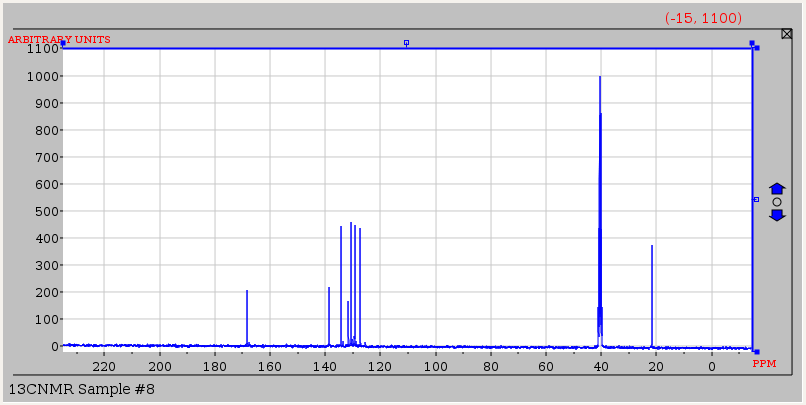
\includegraphics[height=5cm]{figures/CNMR.png}
  \caption{$^{13}$C NMR of \textit{Sample 8}.}
  \label{fig:CNMR}
\end{figure}

\begin{table}[h]
\small
  \caption{$^{13}$C NMR identified peaks for spectra shown in Figure \ref{fig:CNMR}.}
  \label{table:MS}
  \begin{tabular*}{0.5\textwidth}{@{\extracolsep{\fill}}lll}
    \hline
    Peak(s) shift(s) ppm & Designation \\
    \hline
    22 & Methyl carbon \\
    40 & DMSO solvent\\
    130-140 & 6x Aromatic carbons\\
    168 & Carboxylic carbon\\
    \hline
  \end{tabular*}
\end{table}

\section{$^{1}$H NMR}

\begin{figure}[h]
\centering
  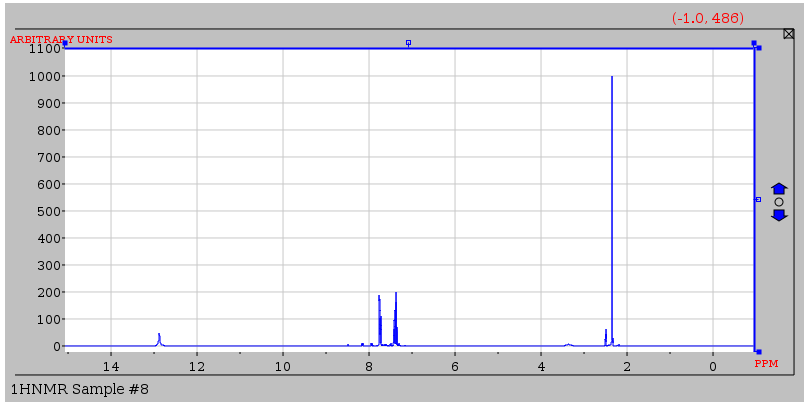
\includegraphics[height=5cm]{figures/HNMR.png}
  \caption{$^{1}$H NMR of \textit{Sample 8}.}
  \label{fig:HNMR}
\end{figure}

\begin{table}[h]
\small
  \caption{$^{13}$C NMR identified peaks for spectra shown in Figure \ref{fig:HNMR}.}
  \label{table:HNMR}
  \begin{tabular*}{0.5\textwidth}{@{\extracolsep{\fill}}llll}
    \hline
    Peak(s) shift(s) ppm & Integration & Splitting & Designation \\
    \hline
    2.3 & 3.1 & Singlet & Ar-CH$_3$ hydrogens\\
    2.4 & 0.4 & Pentet & DMSO\\
    7.35 & 1.1 & Singlet & Aromatic H\\
    7.4 & 1.0 &  Meta Doublet & Aromatic H\\
    7.72 & 1.1 & Meta Doublet & Aromatic H\\
    7.75 & 1.1 & Singlet & Aromatic H\\
    12.8 & 1.0 & Singlet & Carboxylic H\\
    \hline
  \end{tabular*}
\end{table}

\section{Equations}

% an example of a two-column figure
%% \begin{figure*}
%%   \centering
%%   \includegraphics[height=3cm]{example.jpg}
%%   \caption{An example figure caption, an image from the \textit{Physical Chemistry Chemical Physics} cover gallery.}
%%   \label{fgr:example}
%% \end{figure*}

% an example of a two-column table
%\begin{table*}
%\small
  %\caption{\ An example of a caption to accompany a table, table captions do not end in a full point}
  %\label{tbl:example}
  %\begin{tabular*}{\textwidth}{@{\extracolsep{\fill}}lllllll}
    %\hline
    %Header one & Header two & Header three & Header four & Header five & Header six  & Header seven\\
    %\hline
    %1 & 2 & 3 & 4 & 5 & 6  & 7\\
    %8 & 9 & 10 & 11 & 12 & 13 & 14 \\
    %15 & 16 & 17 & 18 & 19 & 20 & 21\\
    %\hline
  %\end{tabular*}
%\end{table*}


%The \balance command can be used to balance the columns on the final page if desired. It should be placed anywhere within the first column of the last page.

%\balance

%If notes are included in your references you can change the title from 'References' to 'Notes and references' using the following command:
%\renewcommand\refname{Notes and references}

\footnotesize{
\bibliography{rsc} %your .bib file
\bibliographystyle{rsc} %the RSC's .bst file
}

\end{document}
